\documentclass[a4paper,11pt]{article}

\usepackage{oikos}
%% Useful packages
\usepackage{amsmath}
\usepackage{graphicx}
\usepackage[colorinlistoftodos]{todonotes}
\usepackage[colorlinks=true, allcolors=blue]{hyperref}
%% Add the following packages in the oikos.sty file
\usepackage{textcomp}
\usepackage{mfirstuc}

%% new commands
\newcommand{\species}[1]{(\xmakefirstuc{\emph{#1}})}

%% Information about the paper

\title{Assessing the timing of territoriality and rutting behaviour in
  roe deer from GPS data}

\author{Morellet Nicolas, Bonenfant Christophe, Miele Vincent,
  \ldots\\ \& Hewison A.J. Mark}

\affiliations{ Christophe Bonenfant, Vincent Miele and Jean-Michel
  Gaillard, Université de Lyon, Université Lyon 1, CNRS, UMR5558,
  Laboratoire de Biométrie et Biologie {\'E}volutive, Bâtiment
  G. Mendel, 43 boulevard du 11 novembre 1918, F-69622, Villeurbanne,
  France - e-mail addresses: christophe.bonenfant@univ-lyon1.fr
  (Christophe Bonenfant); miele.vincent@univ-lyon1.fr (Vincent Miele);
  jean-michel.gaillard@univ-lyon1.fr (Jean-Michel Gaillard) --
}

\begin{document}
%% set on/off for double spacing
%\doublespacing
\maketitle

\newpage
\begin{abstract}
Nice abstract here
\end{abstract}

\newpage
\section*{Introduction}

Mating and reproduction affect many facets of an individual phenotype,
changing its appearance and shape or shaping its life history and
behaviour \citep{Darwin1871}. \todo{Ajoute un commentaire} Across
species the mating system is associated with a set of behaviours
aiming at pairing individuals with sexual partners and increasing
their reproductive success
\citep{Emlen1977,Clutton-Brock1989a,Wittenberger1979}. Males of
polygynous species frequently engaged into intense male-male fights,
do not provide parental care to offspring and are often larger in size
than females. In monogamous species, parents of the two sexes do care
for the offspring, females chose their mating partner carefully and
males often show display courtship behaviour (ref). Mating behaviour
may also vary among populations or individuals of the same species
\citep{Lott1991,Dunbar1982}. The environmental context such as
population density or resource distribution can modulate what mating
behaviour is expressed by most males (Verner and Willson 1966; Caranza
et al. 1990). At the individual level, age, social status, body size
or physiological states are tightly linked with the decision to
reproduce and the type of mating tactic to be adopted. Being closely
associated to reproductive success and fitness, mating and
reproductive behaviours are under strong selection pressures and have
received a lot of attention from ecologists. A careful understanding
of the evolution of reproductive tactics and of mating systems hence
requires to assess if, when, where and how long an individual did
display reproductive-related behaviours.

Many species may, however, be secretive, inhabiting environments with
poor visibility or present a nocturnal activity, so that
reproductive-related behaviours are difficult to observe directly or
to quantify accurately \citep{maher_definitions_1995}. For instance, we
currently have a huge gap of knowledge in the reproductive behaviour
of XXX and XXX because of the observation limitation imposed by the
species lifestyle and its habitat preferences. In this context,
indirect measures, like display of agonistic interactions monitored by
individual acoustic \citep{petruskova_repertoire-based_2016} or spatial
organization can be quantified in order to infer a territorial status
\citep{wronski_home-range_2005,corlatti_hormones_2012} or to assess
whether an individual engaged into reproduction or not. GPS systems
and activity sensors provide powerful new tools to ecologists for
remote monitoring of spatial behaviour
\citep{cagnacci_animal_2010,kie_home-range_2010,kays_terrestrial_2015}. These
devices provide intensive data acquisition with which to infer
behavioural patterns previously impossible or very difficult to
describe exhaustively from direct observation, particularly in closed
or remote and hard to access habitats. For example, in females of
large herbivores parturition date and its fawn survival over the
following weeks were inferred from sudden change in movement speed
(caribou \species{Rangifer tarandus}: ref; white-tailed deer
\species{Odocoileus hemionus}: ref; red deer \species{Cervus elaphus}:
ref). Similarly, Silva et al. (2017) described different lekking
behaviours among little bustard males \species{Tetrax tetrax} from GPS
locations. In marine mammals, locations of animals is frequently used
to define foraging areas of predators such as seals or large seabirds
(). Denning dates were derived from the first date with no-movement of
black bears (). Assuming that a behaviour is associated to a change in
space use, movement or activity, this behaviour should be observable
and detected in the fine-scale locations patterns of individuals (see
Table 1).

Mating is a strong driver of changes in the behaviour of individuals
during the breeding season, including their movements and
activity. Depending on female spatial distribution, males my adopt
different mating tactics (Clutton-Brock 1989) implying specific
movement patterns. For species living at low density with widely
dispersed females such a large carnivores, roaming and greater
movements to find receptive mates during the mating period is a
behaviour that is expressed by many species (monkey, bears). Males may
also engage into the defence of territories overlapping home ranges of
one or several females. Territorial behaviour often results in an
“aggressive behaviour that occurs repeatedly as a direct response to
the location of other individuals, with associated submissive
behaviour on the part of those individuals or groups to which the
aggression is directed” \citep{pyke_territoriality_1996}. In addition
to these marking and agonistic behaviours, territoriality potentially
affects the ranging behaviour and movement of males. Home range of
territorial males are smaller and with a higher density than home
ranges of floaters (Brown et al. 2000). In chimpanzees patrolling
males displayed long-distance movement steps and head-directed
movements, which opposed with the more homogenous movement patterns of
lactating females (Bates and Burns 2009). Similarly, male and females
polar bear displayed contrasting movement parameters attributed to
their roaming and patrolling behaviours, respectively. By eliciting
particular movements of males, mating related behaviours should
therefore be detectable indirectly from movements or space use of
individuals.

The roe deer \species{Capreolus capreolus} is a weakly polygynous
large wild herbivore that inhabits most forests of Europe (Andersen et
al. 1998). Drivers of female reproduction and the reproductive tactics
of female roe deer are relatively well known
\citep{andersen_social_1998} and fine-scale mating behaviours has been
documented recently such as mating excursions
\citep{debeffe_one_2014}. Much less is known about male mating tactics
and behaviours. The mating system of roe deer has been described as
mate defence polygyny \citep{vanpe_mating_2008} where males defend a
mating territory from early spring through the mid-summer rut, when
fertilization of females take place. While reports suggest that most
males become territorial during their fourth summer, some high quality
individuals may successfully mate at 2.5 years old
\citep{vanpe_age-specific_2009}. Hence, despite a relatively low level
of sexual dimorphism, patterns of spatial behaviour differ markedly
between the sexes, as males only are seasonally territorial, while
females do not actively defend their home range \citep[but
see][]{maublanc_ranging_2012}. Territoriality patrolling (Cumming
1966), changes in HR size and scent marking
\citep{gosling_reassessment_1982}. During the rut roe deer males
actively search for females, rub antlers or chase and fight with
competitors generating an increase in the overall activity of animals.

Here, we used a large sample of GPS-monitored roe deer in two
intensively monitored populations in France and Germany to infer
territorial behaviour of male roe deer at both the individual and the
population levels. More specifically, we generated metrics of movement
and activity from GPS locations and activity sensors within the
collars and analysed the temporal patterns of these metrics in
relation to current knowledge on the seasonality of territorial
behaviour in this species \citep{andersen_social_1998}. In particular,
we expected to observe signals of territorial behaviour from early
spring to mid-summer ($i$) in males, but not females
\citep{andersen_mating_1998}, and ($ii$) mostly in prime-age males,
but not sub-adults or yearlings \citep{vanpe_age-specific_2009}. While
high intensity GPS data have previously been used to infer behaviours
such as parturition (\textit{e.g.} \cite{demars_inferring_2013} in
caribou; \cite{asher_use_2014} in red deer; \cite{severud_using_2015}
in moose; \cite{walsh_estimating_2016} in wolves), foraging
\cite{evans_foraging_2013} in common murres) and predation \citep[][
in bears]{krofel_use_2013,cristescu_predicting_2015}, this is, to our
knowledge, the first time that territorial and rutting behaviours has
been inferred from remote GPS monitoring \citep[but see][on lekking in
little bustards]{silva_spatial_2017}.

\section*{Material and Methods}
\subsection*{Study areas}

To assess the timing of territoriality and rutting behaviour in roe
deer, we used the extensive GPS monitoring studies from two sites
which feature in the EURODEER database \citep{cagnacci_partial_2011}. We
selected these study sites (Fig. 1) because they had large sample
sizes for animals of both sexes and all three age-classes (see below).

The study site in the Comminges region of south-west France (N 43° 13',
E 0° 52', 110 km$^2$, hereafter AUR) is a hilly (max. 380 m a.s.l.) mixed
landscape of open fields and small woodland patches, with two large
forests (672 and 463 ha) and numerous small forest patches (covering
19.3\% of the site). The remainder of the study site consists
essentially of meadows for livestock grazing (37.2\%), crops (31.6\%),
and hedgerows (3.6\%). The human population is present throughout the
site, in small villages and farms that are distributed along the
extensive road network. The climate is oceanic, with an average annual
temperature of 11-12° C and 800 mm precipitation. The roe deer is
hunted by stalking during summer (June-August) and drive hunts with
dogs during autumn-winter (September to February).

The study site in Germany and the Czech republic (N 49° 01', E 13° 40',
3070 km², hereafter BAV) is a central European sub-mountainous forest,
including two adjacent National Parks, the Bavarian Forest National
Park (240 km$^2$) and the Šumava National Park (640 km$^2$) in Germany and
Czech republic respectively (D:49° N). There is marked variation in
elevation between 600 and 1450 m a.s.l. and the site consists
essentially of forests of Norway spruce \species{picea abies L.}. The climate
is continental, with an average annual temperature between 3°C and
6.5° C depending on elevation, and an average annual precipitation of
between 830 and 2230 mm. The roe deer is hunted...\todo{to be
  completed by Marco}

\subsection*{Data collection}
For the AUR study site, from 2002-2013, roe deer were caught during
winter (from November 16th to March 27th) using drives of 30-100
beaters and 4 km of long-nets at one of 10 capture sites. For the BAV
study site; from 2004-2015, roe deer were caught during winter
(October–March) using wooden box traps. Each roe deer was sexed and
aged at capture (juveniles ca. 6-10 months old, yearlings ca. 18-22
months old, adults $\geq$ 30 months old), we recorded also its weight
(with an electronic balance to the nearest 0.1 kg). Juveniles are
distinguishable from older deer by the presence of a tricuspid third
pre-molar milk tooth \citep{ratcliffe_roe_1992}, while yearlings can
be quite reliably identified from the degree of tooth wear
\citep{hewison_tests_1999}. Then, deer were equipped with GPS collars
(mainly Lotek 3300 for AUR and Vectronic Aerospace for BAV) and
released on site.

\subsection*{Data processing}
We first selected and standardised location data among the two study
sites. We removed all locations recorded during the first week of
monitoring after an animal’s capture and release because of potential
behavioural alterations following capture and handling
\citep{morellet_effect_2009}. Because the sampling regime of GPS
locations differed among and within study sites, we selected a
comparable number of locations per unit time for each individual
\citep{morellet_seasonality_2013}. We split the day into four periods
of six hours ([0-6[, [6-12[, [12-18[ and [18-0[) and retained the
location that was closest to the beginning of the interval for each
six hour period (\textit{i.e.} a maximum of four locations per day,
with a fix interval of approximately 6 hours). We considered six
months of monitoring as the minimum to obtain a representative
estimate of ranging behaviour over the spring-summer period and we
kept only those individuals with at least 75\% (or 90\%) of the
scheduled locations. The final sample comprised 67 individuals at BAV
and 180 individuals at AUR (or 40 and 90) (average of 3.6 and 3.8
locations per day for 75\% and 90\% of scheduled locations
respectively).

In order to identify temporal changes in behaviour, we generated four
metrics of movement and activity expected to index a territorial
behaviour. As territorial species are known to perform movements in
order to detect potential intruders, to patrol borders, and to
reinforce territory ownership through marking behaviour directed
towards neighbours and peripheral individuals (Owen-Smith, 1977), we
expected an increase of the general mobility and activity for
individuals delimiting a territory. Then, first to describe intensity
of mobility for each individual, we calculated the residence time
\citep{barraquand_animal_2008} and the movement speed of each
individual and expected respectively a decrease of the residence time
and an increase of the speed of territorial individuals so as to
define and maintain a territory. Residence time describes how animals
alternate between intensive (area-concentrated) and extensive (ranging
and relocation) search modes, which are assumed to correspond to
intra-patch and inter-patch movements, respectively. We applied this
approach using a radius of 250 m so that each GPS location is
associated with an estimate of the residence time, which corresponds
to the amount of time spent in the vicinity of any location
\citep{barraquand_animal_2008}. To measure movement speed, we
calculated the straight-line distance between consecutive GPS
locations and divided by the time elapsed. For estimating speed, we
excluded any data where the inter-fix interval was greater than 6
hours. Second, to describe intensity of activity for each individual
we used integrated activity sensors within the GPS collars and
expected an increase of activity, as already mentioned, of territorial
individuals so as to define and maintain a territory. These sensors
measure the frequency of head movements in the horizontal (X) and
vertical (Y) planes over each five minute interval. In order to link
the activity data with the location data in a comparable time series,
we aggregated the activity information across a six hour window
centred on each theoretical GPS location (\textit{i.e.} at 00:00,
06:00, 12:00 and 18:00). For example, for a location obtained at
06:00, we averaged activity data measured from 03:00 to 09:00
separately for both the X and Y axes.

\section*{Statistical analyses}
\subsection*{At the population level}
To detect territorial and/or rutting behaviour, we compared the
movement and activity metrics of male and female juveniles, yearlings
and adults. Indeed, a priori, we expected to observe signals of
territorial behaviour in males but not females, and mostly in
prime-age males, rather than sub-adults or yearlings For the analysis,
we considered the animal’s age as it related to the rut, that is,
animals captured in winter as juveniles are yearling during the
subsequent rutting period (the second of their life), yearlings at
capture become sub-adults (third rut of their life), while adults at
capture remain adult during the subsequent rutting event.

We analysed the temporal patterns of the four metrics, i.e. residence
time in a radius of 250 m (RT250), movement speed (speed), mean head
movements on the X axis (meanX) and on the Y axis (meanY). We used
generalised additive mixed models (GAMMs) to model these four
dependant variables separately, including roe deer identity as a
random factor to control for repeated observations per individual. We
used GAMM rather than standard linear models because GAMMs capture
nonlinear temporal variation more efficiently. We used cyclic
P-splines to smooth the effect of time to account for the cyclic
pattern of the dependant variables over the year. Because day length
influences the ranging behaviour of roe deer
\citep{borger_integrated_2006}, we arbitrarily set the winter solstice
(December 22nd) as the common starting day (Julian date = 1) for both
study sites \cite[see also][]{morellet_seasonality_2013}. We included
sex (two modalities), age class (three modalities) and study site (two
modalities) as explanatory factors. For each dependent variable
separately, we compared five models: a model containing only the
spline of the Julian date (baseline model), a model including a
sex-specific temporal effect (i.e. a spline of Julian date for each
sex), a model including both a sex-specific and age-specific temporal
effect, a model including a sex-specific and a site-specific temporal
effect, and a model including a sex-specific, age-specific and
site-specific temporal effect. We systematically included sex in all
models other than the baseline model as there was a strong a priori
reason to expect the temporal pattern should differ between sexes (see
above). In order to improve the quality of the fit of GAMM models and
then to reduce the structure of residuals, we used the Box-Cox power
transformation of the four variables using the boxcox function in the
\textit{MASS} library implemented in R software, version 3.3.1 (R Core
Team, 2016). We used the second order Akaike’s information criterion
corrected for small sample size \citep[AICc][]{burnham_model_1998} and
Akaike weights ($w$) to select the model with the most support among
the set of five candidate models constructed a priori. All generalized
additive mixed models were fitted using the “gamm” function in the
\textit{mgcv} library \cite{wood_generalized_2006} in \textbf{R}
software.\todo{penses-tu qu'il soit nécessaire d'expliquer que nous
  avons augmenter le lissage} Finally, because the inclusion of
non-sedentary animals might influence the analysis, to evaluate the
robustness of our results, we eliminated all individuals that were not
classified as sedentary following the approach described in
\cite{cagnacci_partial_2011} and then repeated the analyses.

\subsection*{At the individual level}
To see whether it is possible to discriminate territorial and
non-territorial animals, we used an unsupervised clustering method
based on the three temporal metrics speed, meanX and meanY. We did not
consider RT250 at this stage as this metric was less informative at
population level (see Results). We performed a hierarchical
clustering, a classical technique that groups individuals together if
they present similar temporal metrics. This method requires a single
distance matrix computed on the basis of the three metrics:
consequently, for any pair of individuals, we computed the quadratic
mean of 1/ the distance between the two speed metrics and 2/ the
distance between the two activity metrics (meanX and meanY taken
together) of this pair of individuals. Since the temporal metrics can
be highly fluctuating between subsequent locations, the distance
between the metrics of two individuals can be overestimated due to
irrelevant fine scale variations. To circumvent this issue, we
previously denoised and smoothed the temporal metrics one by one with
wavelets (from an original metrics, we retained the inverse discrete
wavelet transform with the lowest frequency levels as the metrics to
be considered in the clustering approach; R package
\textit{wavethresh} REF=tps://www.springer.com/us/book/9780387759609)
and we standardized the metrics. From the hierarchical clustering
results, we deduced the partition of the individuals into two groups
of similar metrics.

As territorial status was unknown, we evaluated the composition of
these groups in terms of sex and age classes since only males are
expected to be territorial and mostly adults. As we generated two
groups of individuals (see Results), we performed generalized linear
models with a logit link function to analyse groups in relation to sex
(male versus female), study site (AUR versus BAV) and age class
(yearlings, sub-adults and adults). As we expected to observe the
territorial behaviour mostly on adult roe deer and in order to make
sure we obtained the same results over the two sites, we included also
the three-way interactions between these sex, site and age class (and
all two-way interactions) in the most complex model. Due to missing
data for the hierarchical clustering of some individuals, sample size
for this analysis (individuals with at least 75\% of the scheduled
locations) was 52 and 168 individuals for BAV and AUR,
respectively.\todo{On n'a pas le même nombre d'individus à l'issu du
  clustering} To identify the best supported model, we again used the
second order Akaike’s information criterion corrected for small sample
size.

We used the \textit{dredge} function in the \textit{MuMIn} library to
generate all sets of models \citep{barton_mumin:_2016}.

\section*{Results}
\subsection*{At the population level}

Our overall results were robust with respect to sedentary
status. Indeed, whether we restricted the analysis to sedentary
individuals only, or analysed all available individuals, the results
were comparable (see Electronic Appendix S1). Thus, here we present
results based on the whole data set.

Residence time (RT250), movement speed (speed), mean head movements on
the X axis (meanX) and on the Y axis (meanY) all showed strong
temporal variation that differed in amplitude, timing and general
pattern among sexes, age classes and study sites (AICc weight = 1,
Table 1). In males, except for residence time, the temporal variation
of the different metrics followed a comparable pattern
(Fig. 2). However, the temporal variation of the four metrics differed
markedly between adult males and females (Fig. 2). Residence time of
females showed a pronounced peak shortly after the birth period,
whereas it was more or less constant for males. These temporal
fluctuations were generally more pronounced for adults compared to
yearlings and sub-adults (Fig. 3).

For females, movement speed followed an inverted bell curve, and was
highest during winter and lowest near the summer solstice. However,
the temporal variations in actvity (head movements on the X and Y
axes) were not very consistent between the two study sites. In
contrast, for males, both movement speed and head movements (X and Y
axes) followed a bimodal distribution, with one peak in spring (around
the 20th of April and 1st of May for AUR and BAV, respectively) and
another peak in summer (around the 1st of August and 25th of July for
AUR and BAV, respectively).

\subsection*{At the individual level}
From the hierarchical clustering performed separately for each study
site on movement speed and head movements (meanX+meanY), for each
study site we retained two clusters of individuals that showed
comparable temporal patterns (see Electronic Appendix S2). One cluster
included all individuals that had two temporal peaks for movement
speed and head movements (cluster 2), the other cluster contained
individuals that showed an inverted bell curve in movement speed (with
a higher speed during winter than during summer) and only one temporal
peak (see Electronic Appendix S2). In the next step, we thus
considered individuals with two pronounced activity peaks as those
most likely to be engaged in territorial behaviour. In the analysis of
the sex-, study site- and age- dependence of this behaviour, the best
model describing the probability of having two activity peaks
contained only the two-way interaction between age and sex (AICc
weight = 0.25, Table 2, Fig. 4). The probability of having two
activity peaks was much lower for adult females (0.016$\pm$0.016) than for
adult males (0.852$\pm$0.048).

\section*{Discussion}

\bibliography{nico,/home/christophe/Documents/bibtex/Kris_2006}

\newpage
\begin{table}[htbp]
  \centering
  \caption{Performance of the five candidate generalized additive
    mixed models for residence time in a radius of 250 m (RT250),
    movement speed (speed), mean head movements on the X axis (meanX)
    and the Y axis (meanY), including a smoothed effect of time
    (Julian date) based on a cyclic P-spline, which differed between
    sexes, between sexes and age classes, between sexes and study
    sites, and between sexes, age classes and study sites, for
    individual roe deer with at least 75\% of scheduled locations in
    the two study sites (AUR in France and BAV in Germany), from 2002
    to 2013 in AUR and from 2004 and 2015 in BAV. The most supported
    model, based on the differences in the values for $\Delta$AICc and Akaike
    weights ($w$), is reported in bold. All models including a two-way
    interaction also include main effects. AICc is the value of the
    corrected Akaike’s information criterion and df is the number of
    degree of freedom for each model.}
  
    \begin{tabular}{rrrrrr}
      \\
      \hline  
      Proxy & Models & df    & AICc  & $\Delta$AICc & $w$ \\
      \hline
      RT250 & S(time) & 266.6 & -703224.5 & 31710.8 & <0.001 \\
            & S(time by sex) & 285   & -720677.4 & 14257.9 & <0.001 \\
            & S(time by sex, age) & 355.9 & -724606.7 & 10328.6 & <0.001 \\
            & S(time by sex, study & 321.5 & -728284.1 & 6651.2 & <0.001 \\
            & \textbf{S(time by sex, age, study} & \textbf{461.4} & \textbf{-734935.3} & \textbf{0} & \textbf{1} \\        
      \hline
      Speed & S(time) & 262.4 & 335783.2 & 8361.3 & <0.001 \\
            & S(time by sex) & 278.2 & 331056.5 & 3634.6 & <0.001 \\
            & S(time by sex, age) & 339.7 & 329990.8 & 2568.9 & <0.001 \\
            & S(time by sex, study & 314.6 & 328918.7 & 1496.9 & <0.001 \\
            & \textbf{S(time by sex, age, study} & \textbf{432.7} & \textbf{327421.8} & \textbf{0} & \textbf{1} \\
      \hline
      MeanX & S(time) & 237.8 & 1001934.3 & 24639.5 & <0.001 \\
            & S(time by sex) & 256.5 & 996264.1 & 18969.3 & <0.001 \\
            & S(time by sex, age) & 329.3 & 993102.3 & 15807.5 & <0.001 \\
            & S(time by sex, study & 293.7 & 981784.4 & 4489.6 & <0.001 \\
            & \textbf{S(time by sex, age, study} & \textbf{438.2} & \textbf{977294.8} & \textbf{0} & \textbf{1} \\       
      \hline
      MeanY & S(time) & 237.6 & 1125826.3 & 19234.9 & <0.001 \\
            & S(time by sex) & 256.3 & 1121643.1 & 15051.7 & <0.001 \\
            & S(time by sex, age) & 327.4 & 1119574.2 & 12982.8 & <0.001 \\
            & S(time by sex, study & 293.7 & 1109759.4 & 3168  & <0.001 \\
            & \textbf{S(time by sex, age, study} & \textbf{433.5} & \textbf{1106591.4} & \textbf{0} & \textbf{1} \\
      \hline 
    \end{tabular}
  \label{tab:addlabel}
  \end{table}
 
\begin{table}[t]
  \centering
  \caption{Summaries of the candidate generalized linear models to
    investigate the probability of having two activity peaks in
    relation to sex, age class and study site, and the three-way
    interaction between sex, age class and study site, for individual
    roe deer with at least 75\% of scheduled locations in the two
    study sites (AUR in France and BAV in Germany), from 2002 to 2013
    in AUR and from 2004 and 2015 in BAV. We only report the
    top-ranked model with a $\Delta$AICc that differed by < 5 from the most
    supported model in the table (in bold) and the null model. All
    models including a two-way interaction also include main
    effects. AICc is the value of the corrected Akaike’s information
    criterion and df is the number of degree of freedom for each
    model. The ranking of the models is based on the differences in
    the values for $\Delta$AICc and Akaike weights ($w$).}
  
    \begin{tabular}{rrrrr}
    \\
    \hline
        Models & df    & AICc  & $\Delta$AICc & $w$ \\
    \hline
    \textbf{sex x age} & \textbf{6}     & \textbf{172.1} & \textbf{0}     & \textbf{0.253} \\
    sex x age  + site x sex & 8     & 172.4 & 0.31  & 0.217 \\
    sex x age + age x site & 9     & 172.6 & 0.47  & 0.2 \\
    sex x age + site & 7     & 172.9 & 0.74  & 0.175 \\
    sex x age + age x site + sex x site & 10    & 173.1 & 0.97  & 0.156 \\
    Null  & 1     & 293.6 & 121.48 & 0 \\
    \hline
    \end{tabular}
  \label{tab:addlabel}
\end{table}

\newpage
\begin{figure} [ht!]
  \centering
  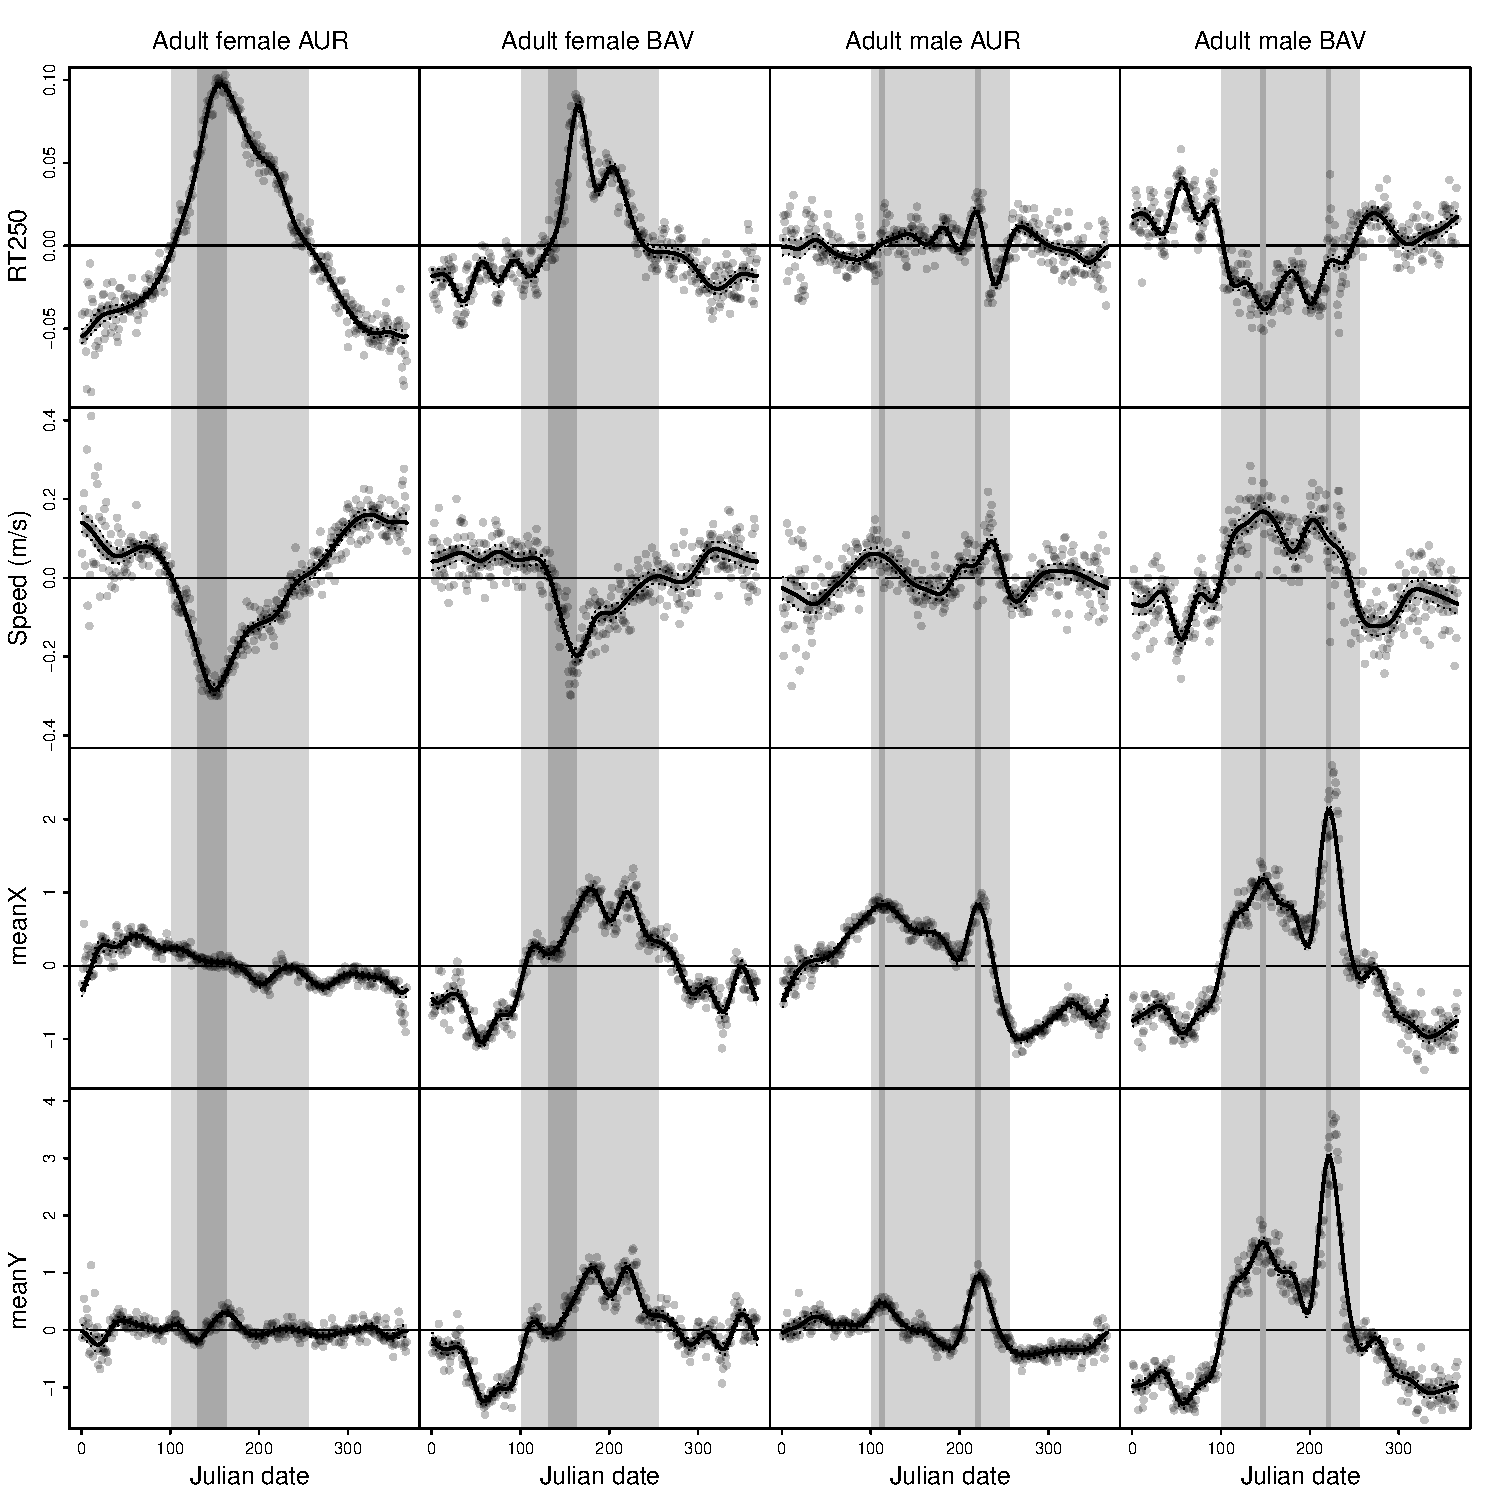
\includegraphics[width=0.9\linewidth]{./figures/Fig2NB.pdf}
  \caption{Temporal variations in residence time within a radius of
    250 m (RT250), movement speed (speed), mean head movements on the
    X axis (meanX) and mean head movements on the Y axis (meanY) for
    adult male and female roe deer in the two study sites (AUR in
    France and BAV in Germany), from 2002 to 2013 in AUR and from 2004
    and 2015 in BAV. The time series starts on the 22nd of
    December. The lines (and dotted lines) represent the separate GAMM
    models for each variable (with the confidence intervals) including
    a smoothed effect of time (Julian date) based on cyclic P-spline,
    which differed among study sites, sexes and age classes. Based on
    the literature, the light gray represents the assumed territorial
    period, from the 1st of April to the 1st of September, and the
    dark gray represents the birth period for females, from the 1st of
    May to the 1st of June. Finally, for males the dark gray lines
    represent the temporal window for the observed peaks in these
    metrics in spring (20th of April and 1st of May for F:43° N and
    D:49° N, respectively) and summer (1st of August and 25th of July
    for F:43° N and D:49° N, respectively).}
\end{figure}

\newpage
\begin{figure} [!h]
  \centering
  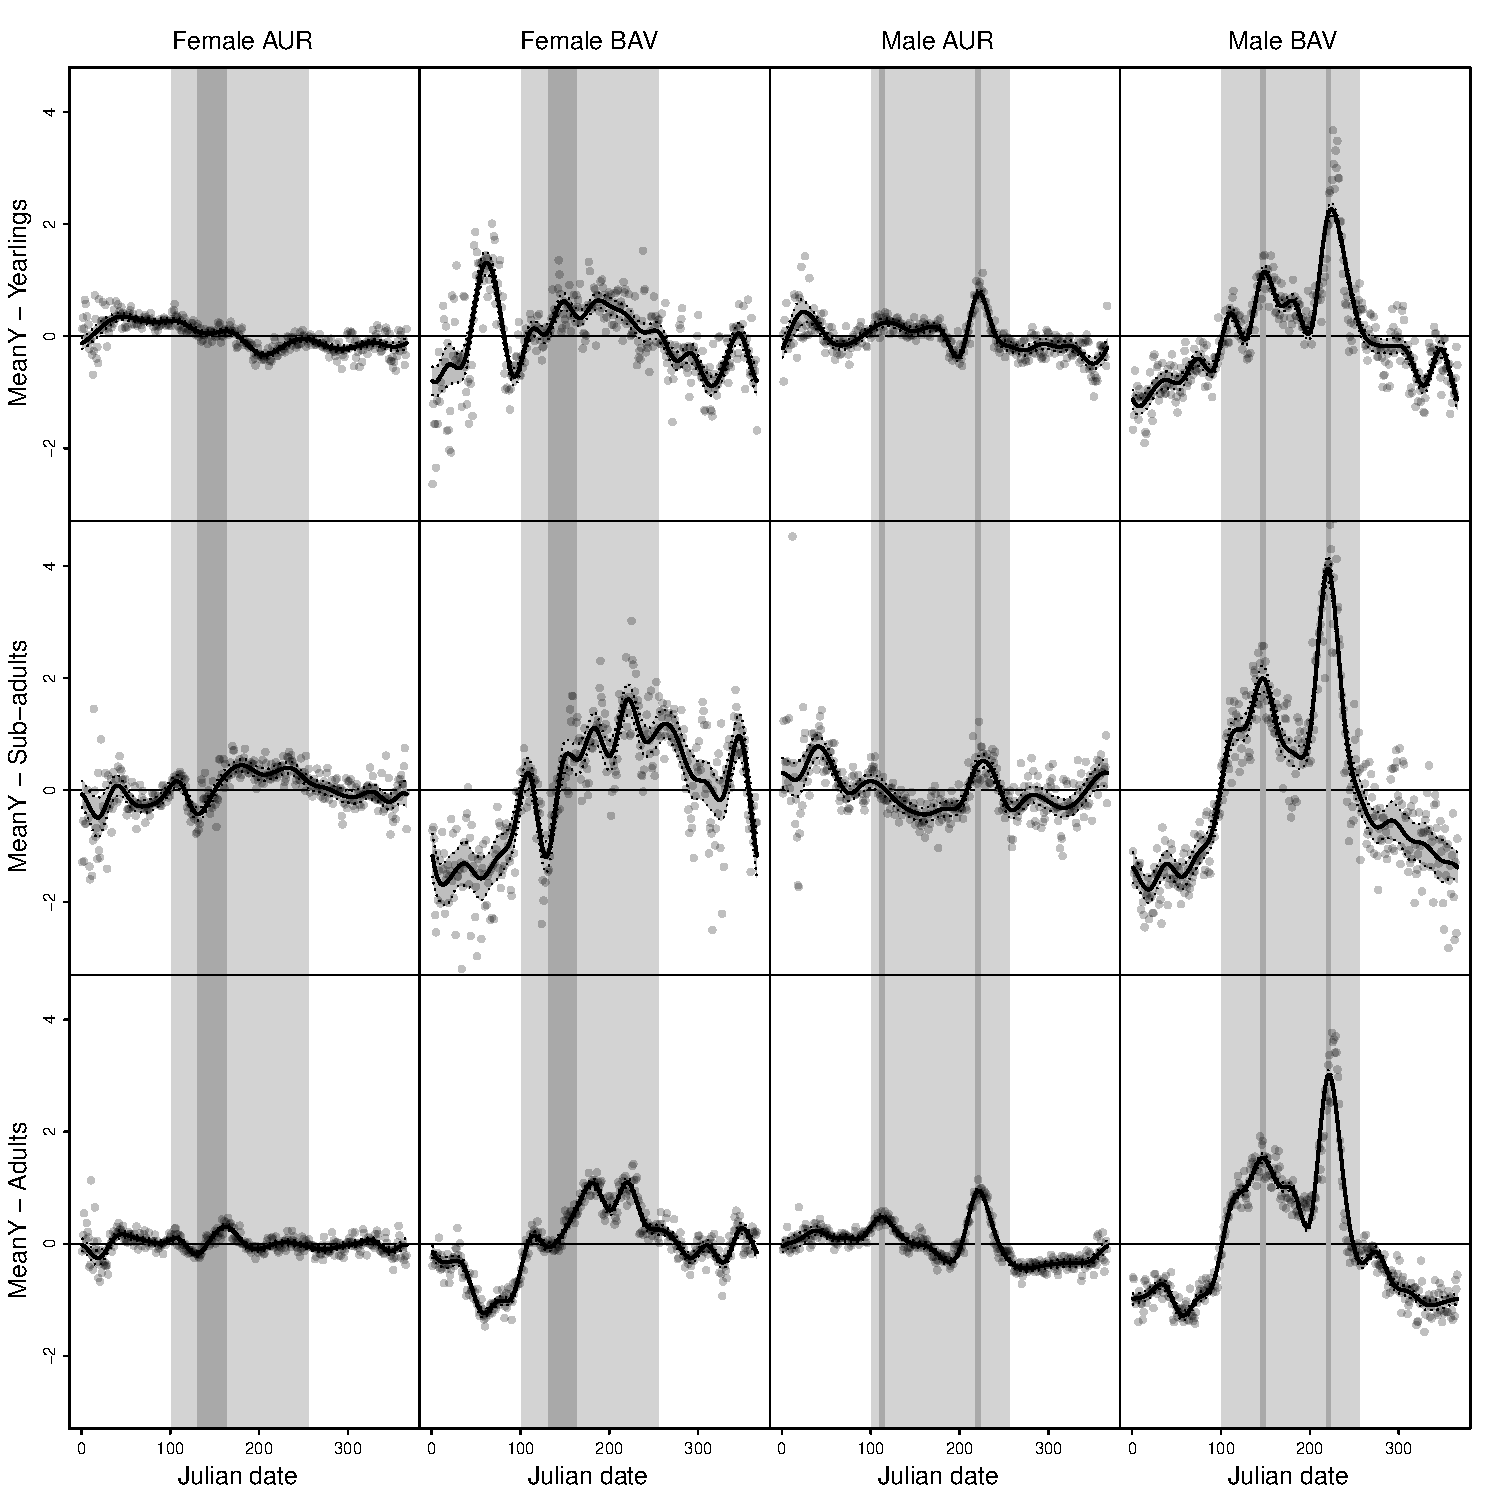
\includegraphics[width=0.9\linewidth]{./figures/Fig3b.pdf}
  \caption{Temporal variations in mean head movements on the Y axis
    for male and female roe deer among age classes in the two study
    sites (AUR in France and BAV in Germany), from 2002 to 2013 in AUR
    and from 2004 and 2015 in BAV. The time series starts on the 22nd
    of December. The lines (and dotted lines) represent the GAMM
    models (with the confidence intervals) including a smoothed effect
    of time (Julian date) based on a cyclic P-spline, which differed
    among study sites, sexes and age classes. Based on the literature,
    the light gray represents the assumed territorial period, from the
    1st of April to the 1st of September, and the dark gray represents
    the birth period for females, from the 1st of May to the 1st of
    June. Finally, for males the dark gray lines represent the
    temporal window for the observed peaks in these metrics in spring
    (20th of April and 1st of May for F:43° N and D:49° N,
    respectively) and summer (1st of August and 25th of July for F:43°
    N and D:49° N, respectively).}
\end{figure}

\begin{figure} [!h]
  \centering
  \includegraphics[width=0.5\linewidth]{./figures/Fig4.pdf}
  \caption{The probability of having two temporal peaks of activity in
    relation to the sex and the age class, for roe deer monitored in
    two study sites (AUR in France and BAV in Germany), from 2002 to
    2013 in AUR and from 2004 and 2015 in BAV. The dots (and segment
    lines) represent the GLM models (with the confidence intervals).}
\end{figure}

\end{document}
